\documentclass{article}

\usepackage{packages}
\usepackage{environments}
\usepackage{commands}

% Потребуется для вставки картинки подписи
% \usepackage{graphicx}

\usepackage{titlepage}

% Здесь задаем параметры титульной страницы
% Выбрать одно из двух
%\setToResearch
\setToProgram

\setTitle{3D рендерер с нуля}

% Выбрать одно из трех:
% КТ1 -- \setStageOne
% КТ2 -- \setStageTwo
% Финальная версия -- \setStageFinal
\setStageOne
%\setStageTwo
%\setStageFinal

\setGroup{213}
% Сюда можно воткнуть картинку подписи с помощью \includegraphics[scale=0.2]{<имя файла>}
% (scale подбирается индивидуально для конкретной картинки)
% \setStudentSgn{\includegraphics[scale=0.2, trim=-5cm 3cm 0 0]{signature.png}}
\setStudent{Д.С.Бонич}
\setStudentDate{14.02.2023}
\setAdvisor{Дмитрий Витальевич Трушин}
\setAdvisorTitle{доцент, к.ф.-м.н.}
\setAdvisorAffiliation{ФКН НИУ ВШЭ}
\setAdvisorDate{14.02.}
\setGrade{}
% Сюда можно воткнуть картинку подписи с помощью \includegraphics[scale=0.2]{<имя файла>}
% (scale подбирается индивидуально для конкретной картинки)
% \setAdvisorSgn{\includegraphics[scale=0.4]{trushin_signature.jpg}}
\setYear{2023}

% С этого момента начинается текст документа
\begin{document}

% Эта команда создает титульную страницу
\makeTitlePage

% Здесь будет автоматически генерироваться содержание документа
\tableofcontents

% Данное окружение оформляет аннотацию: краткое описание текста выделенным абзацем после заголовка
\begin{abstract}
    Главной целью данной работы является написание своего 
    собственного 3D-рендерера -- программы для отображения трехмерных объектов на плоский 
    экран компьютера.
\end{abstract}


\section{Введение}

\emph{Рендеринг} (англ. rendering -- <<визуализация>>) --- это процесс 
получения изображения из модели, его строгого описания. 
Часто под рендерингом подразумевают 3D-рендеринг, где по 
описанию объектов из $\R^3$ строится плоское изображение,  
готовое к отображению на плоском экране компьютера. Программа 
осуществляющая ренедеринг называется рендерером, а результат её работы 
рендером. В данной работе мы рассмотрим только 3D-рендеринг и 
3D-рендереры.В рендеринге можно выделить два основных 
типа: real-time и offline рендеринг. Real-time рендеринг подразумевает 
быстрый рендеринг изображения, достаточный для создания эффекта движения на 
экране. Этот тип исползуется в видеоиграх, где важно быстро 
рендерить постоянно меняющуюся модель мира. Offline рендеринг 
может требовать минуты, часы или даже дни для производства рендера, 
но как правило это оправдано высоким качеством финального изображения. Нас будет интересовать 
real-time рендеринг. При реализации рендеринга на вычислительных 
устройствах существует 2 принципиально разных подхода. Можно 
осуществлять рендеринг с помощью видеокарты, а можно использовать 
только компьютерный процессор. Первый способ является наиболее 
распространенным для real-time рендеринга.
Причиной этому служат специфичные потребности алгоритмов осуществляющих рендеринг.
Как правило требуется запускать небольшие программы для каждого 
пикселя. В компьютерной графике такие небольшие программы, которые 
можно выполнять параллельно, называют \emph{шейдерами}. Так как 
видеокарта имеет большое количество слабых ядер, она является 
идеальным кандидатом для выполнения шейдеров и сильно выигрывает 
в производительности у процессора. Не смотря на это у второго 
подхода есть свои преимущества. Такой способ рендеринга называется
\emph{программным рендерингом} (software rendering) и может быть 
использован для применения специфичных алгоритмов визуализации, которые 
по каким-то причинам сложно или невозможно реализовать на существующих видеокартах.
Это обусловлено тем, что многие видеокарты фиксируют некоторую 
часть алгоритмов входящих в рендеринг, не позволяя их поменять.
Мы будем использовать программный рендеринг, так как хотим 
реализовать весь пайплайн рендеринга с нуля. Можно добавить еще 
разделение рендереров по основному принципу с помощью которого осуществляется рендеринг. 
Есть методы рассматривающие 
лучи света, а есть \emph{растеризация}. Наш рендерер будет использовать растеризацию. 
Это значит что изначально мы не будем опиратся на свет и будем 
строить все сложные объекты сцены из кирпичиков --- примитивов. 
Основным примитивом для нас будет являтся треугольник. С помощью 
треугольников можно получить или хорошо аппроксимировать любой 
объект в $\mathbb{R}^3$.

Проссумировав все выше сказанное, главной целью проекта является реализация собственного программного real-time 
3D-рендерера, использующего подход растеризации в качестве основы.

Были реализованы следующие фичи:
\begin{itemize}
    \item Растеризация треугольников с соблюдением top-left rule 
    \item Screen-space clipping
    \item Frustrum clipping
    \item Z-buffering
    \item Face culling
    \item Линейная интерполяция значений внутри треугольника с учетом перспективы
    \item Наложение текстур на треугольники с учетом перспективы
    \item Набор функций для осуществления линейных преобразований, сдвигов, а также 
    переходов между различными системами координат 
    \item Загрузка и рендеринг моделей, сцен созданных в программах 3D моделлирования 
    \item Точечный свет 
    \item Phong shading
    % \item Рендеринг текста с помощью TrueType шрифтов
    % \item Реализация программы с использованием MVC паттерна в качестве основы
\end{itemize}

При написании использовалась \href{https://www.youtube.com/watch?v=Y_vvC2G7vRo&list=PLEETnX-uPtBUbVOok816vTl1K9vV1GgH5&index=2}{серия видео} от thebennybox, в ходе 
которых был реализован 3D-рендерер на языке Java. Также для реализации 
корректного наложения текстур ознакомился с серией статей от 
Chris Hecker\cite{Textures}. Остальные более обширные источники указаны в 
списке литературы.

\section{Требования к программе}
\subsection*{Функциональные}
    Программа способна рендерить \href{https://en.wikipedia.org/wiki/Utah_teapot}{utah teapot} с 
    базовым освещением и разрешением 1920x1080. Пользователь программы 
    имеет возможность исследовать заготовленную 3D сцену перемещаясь с помощью мыши и 
    клавиатуры.  

\subsection*{Нефункциональные}
Вся программа целиком написана на C++. Графическая библиотека SFML используется
только для вывода отрендереного изображения на экран.
Также были использованы библиотеки с готовыми математическими классами, например с матрицами 
и векторами. 
Были использованы следующие библиотеки:
\begin{itemize}
    \item \href{https://www.sfml-dev.org/index.php}{SFML} --- для создания окна и вывода изображения на экран 
    \item \href{https://github.com/g-truc/glm}{GLM} --- для классов матрицы и вектора, а также базовых 
    операций с ними
    \item \href{https://github.com/nothings/stb/blob/master/stb\_image.h}{stb\_image.h} --- для загрузки изображений разных форматов в оперативную память
\end{itemize}
Сборка проекта осуществляется с помощью \href{https://cmake.org/}{CMake}.
Для форматирования кода используется \href{https://clang.llvm.org/docs/ClangFormat.html}{ClangFormat}, 
для линтинга и статического анализа \href{https://releases.llvm.org/10.0.0/tools/clang/tools/extra/docs/clang-tidy/index.html#:~:text=clang%2Dtidy%20is%20a%20clang,be%20deduced%20via%20static%20analysis.}{Clang-Tidy}.
Кодстайл основан на \href{https://google.github.io/styleguide/cppguide.html}{Google C++ Style Guide}.
Используемая система контроля версий --- \href{https://git-scm.com/}{git}, удаленный репозиторий 
лежит на \href{github.com}{github}. 

\section{Структура программы}

Рендерер будет включать себя две основные части: графический пайплайн 
и инфраструктура вокруг него позволяющая взаимодействовать с пайплайном. 

\subsection{Обзор графического пайплайна}

Для начала сосредоточимся на задаче рендеринга одного единственного 
треугольника. Для этого нам нужно познакомиться с различными полезными 
системами координат.

\begin{center}
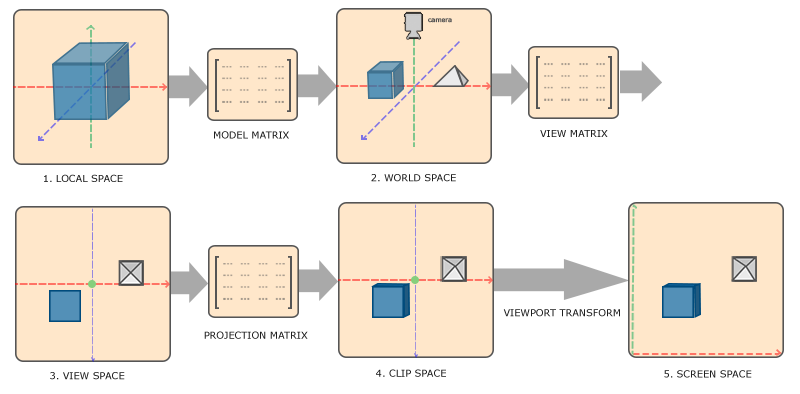
\includegraphics[scale = 0.6]{coordinate_systems.png}

Cхема взята \href{https://learnopengl.com/Getting-started/Coordinate-Systems}{отсюда}
\end{center}

\begin{enumerate}
    \item \textbf{Local space}.
    В этой системе координат мы задаем форму треугольника.
    \item \textbf{World space}.
    Эта система координат говорит нам расположение треугольника в нашей сцене, как 
    он повернут, а также его размер.
    \item \textbf{View space}.
    Эта система координат говорит нам как расположен треугольник 
    относительно наблюдателя, называемого камерой.
    \item \textbf{Clip space}.
    В этой системе координат все <<видимые>> камерой вершины должны 
    попасть в отрезок $[-1, 1]$. 
    \item \textbf{Screen space}. Здесь первые 
    две координаты $x, y$ считаются настоящими координатами пикселей на экране.
\end{enumerate}

Как видно из схемы, мы можем переводить координаты 
точки из одной системы координат в другую, умножая 
соответствующую матрицу слева на вектор координат.

Мы будем задавать координаты точки с помощью вектора 
$\R^4$. Первые три координаты будут отвечать за координаты в 
$\R^3$ и обозначаться $x$, $y$ и $z$ соответственно, а 
последнюю компоненту будем обозначать как $w$. При задании 
координат треугольника в local space мы будем всегда считать 
$w=1$. У этой координаты есть несколько полезных применений. 
Для начала, чтобы преобразовать координаты из local space в 
model space нам может потребоваться <<сдвинуть>> координаты точки на 
некоторый вектор. Но такое преобразование меняет начало координат, а 
значит не может быть линейным в $\R^3$. Работая же в 
$\R^4$ мы можем легко делать подобные аффинные преобразования:

\[
    \begin{pmatrix}
        1 & 0 & 0 & x_{add}\\
        0 & 1 & 0 & y_{add}\\
        0 & 0 & 1 & z_{add}\\
        0 & 0 & 0 & 1
    \end{pmatrix}
    \begin{pmatrix}
        x\\ y\\ z\\ 1\\
    \end{pmatrix} = 
    \begin{pmatrix}
        x + x_{add}\\
        y + y_{add}\\
        z + z_{add}\\
        1
    \end{pmatrix}
\]

Тут мы можем видеть как вектор $(x, y, z)^T$ был 
сдвинут на вектор $(x_{add}, y_{add}, z_{add})^T$.

Помимо сдвигов, при преобразовании из local space в 
world space может также использоваться умножение всех 
координат кроме $w$ на скаляр, а также поворот вектора 
в $\R^3$. Все эти операции являются линейными преобразованиями 
и могут быть выражены с помощью матричного умножения на вектор.

Чтобы перейти из world space к view space нам нужна 
информация о камере. Камера может задаваться её координатами 
в world space и вектором задающим направление в котором 
она смотрит. Из этой информации может быть 
построена view матрица. 

Чтобы перейти от view space к clip space используется 
матрица проекции. Чтобы передать ощущение глубины объектов мы 
будем использовать перспективную проекцию. 

\begin{center}
    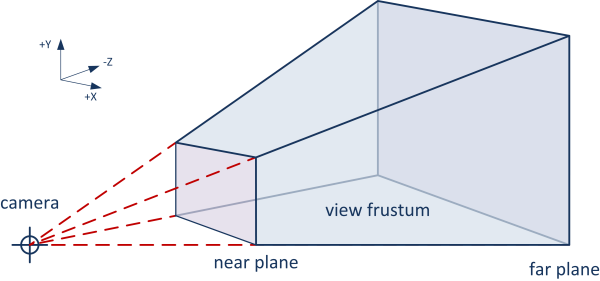
\includegraphics[scale=5]{frustum.png}

    \href{https://learnopengl.com/Guest-Articles/2021/Scene/Frustum-Culling}{Источник}
\end{center}

Договариваемся, что камера смотрит в направлении $-z$, 
$x$ идет вправо от камеры, а $y$ вверх в рамках 
view space.
Суть в том, что только точки попадающие в 
усеченный конус(view frustum) будут отображены. 
Все что находится за пределами view frustum считается
расположеным вне обзора нашей камеры. Усеченный 
конус задается расстоянием до близкой плоскости(near plane), 
расстоянием до далекой плоскости(far plane), соотношением 
ширины near plane к высоте near plane, а также углом 
между левой и правой плоскостями, называемым FOV(field of view).
Зная все это мы можем получить нашу матрицу проекции и перейти в clip 
space.

На самом деле чтобы перейти в clip space нам не достаточно 
просто умножить на матрицу проекции. Дело в том, что 
в этом преобразовании нам требуется поделить координаты, что 
не является аффинным преобразованием. Поэтому матрица проекции 
записывает число на которое нужно поделить все координаты в компоненту 
$w$. Действие деления всех координат вектора на $w$ называется 
perspective division и должно происходить до перехода 
к screen space. Во время перехода к clip space view 
frustum отображается в куб с координатами от $-1$ до $1$. 
Такие координаты называют normalized device coordinates(NDC).

На этой стадии происходит обрезка(clipping). Все вершины 
треугольника находящиеся за пределами куба удаляются, 
при этом добавляются новые вершины чтобы представить 
оставшуюся внутри куба часть треугольника. Такая остаточная 
фигура всегда выпукла, поэтому легко разбивается на треугольники.

Для преобразования из clip space в screen space достаточно 
знать ширину(hl) и высоту(vl) окна в пикселях.
Тогда $x$ и $y$ координаты будут находится в отрезках $[0, hl - 1]$ и $[0, vl - 1]$, 
где целые координаты соответствуют центрам пикселей, ось 
$x$ идет слева направо, ось $y$ сверху вниз.

Для треугольника в screen space выполняется растеризация ---
процесс опредления пикселей на экране принадлежащих треугольнику.
Используемый алгоритм растеризации следующий:

\begin{enumerate}
    \item Отсортируем вершины по возрастанию их $y$ координат и обозначим 
    их в порядке сортировки как $y_{min}, y_{mid}, y_{max}$. Назовем 
    стороны треугольника следующим образом: $y_{min}$-$y_{max}$ -- long edge, 
    $y_{min}$-$y_{mid}$ top edge, $y_{mid}$-$y_{max}$ bottom edge.
    \item Будем двигаться по одному пикселю вниз одновременно на long edge и 
    top edge пока top edge не закончится. На каждом шаге пиксели между long 
    edge и top edge на данной высоте y отмечаем как отображаемые.
    \item Аналогично шагу 2, но теперь берем остаток long edge и bottom edge.
\end{enumerate}

Также при растеризации выполняется линейная интерполяция некоторых значений 
лежащих в вершинах помимо координат. Сюда входят: базовый цвет, нормаль, 
координаты текстуры. Для того чтобы делать 
линейную интерполяцию во время растеризации, казалось бы достаточно вычислить градиент переменной 
которую мы хотим интерполировать. Но проблема в том что если мы делаем эту интерполяцию в 
screen space, то функция задающая значения в произвольных точках треугольника уже 
не линейная. И все это из-за perspective division. Но к счастью можно заметить, что 
зависимость интерполянта деленного на глубину линейна в screen space. Обратное к глубине 
так же линейно, так что интерполируя эти вещи мы можем восстановить значение исходного 
интерполянта в каждой точке.

Освещение обеспечивается точечными источниками света. Свет для 
каждого фрагмента треугольника является по сути вектором цвета умножаемым 
на реальный цвет фрагмента получаемый либо из его базового цвета, либо из 
текстуры. Чтобы посчитать свет для фрагмента используются его координаты в 
world space, позиция камеры в world space, нормаль, а также информация об источнике 
света.  

Чтобы более далекие от камеры треугольники не затирали пиксели 
более близких треугольников используется z-buffering. Это 
экранный буфер, в котором для каждого пикселя сохраняется $z$ координата 
последнего пикселя треугольника который был туда записан. Тогда 
мы записываем цвет пикселя треугольника на экран только если $z$ 
значение пикселя треугольника больше чем соответствующее значение 
в $z$-буфере.

Также можно опционально включить менее общий механизм, позволяющий 
не рендерить целые полигоны, если они не видны наблюдателю. Этот 
механизм называется face culling, но работает не для всех моделей. 
При использовании face culling мы считаем что у каждого полигона есть видимая 
и невидимая сторона. Чтобы определить какая из сторон какая мы используем порядок в 
котором перечислины вершины треугольника. Если они идут против часовой стрелки мы считаем, 
что такая стороно видима и невидима иначе.

\subsection{Устройство инфраструктуры в программе}

Главным классом в исходном коде является Application. Он отвечает 
за главный цикл отрисовки и обработки событий, а также хранит хранит внутри 
себя классы Window, Renderer, Camera используя композицию. Внутреннее представление 
сцены для отрисовки также лежит на нем. 

Класс Window отвечает за создание окна, а 
также предоставляет интерфейс для обработки ввода компьютерной мыши и клавиатуры. 

Класс Renderer отвечает за рендеринг моделей хранящихся в виде экземпляров класса 
Model. Для этого он использует класс PrimitiveRenderer способный рендерить только треугольники.

Класс Camera отвечает за хранение состояния камеры, а также предоставляет 
интерфейс для доступа к этим данным как для чтения, так и для изменения.


\nocite{OpenGLMath}
\nocite{GameMath}
\nocite{CompGraphicsDynamic}
\nocite{CompGraphicsPolyg}
% Здесь автоматически генерируется библиография. Первая команда задает стиль оформления библиографии, а вторая указывает на имя файла с расширением bib, в котором находится информация об источниках.
\bibliographystyle{plainurl}
\bibliography{bibl}

% Здесь текст документа заканчивается
\end{document}
% Начиная с этого момента весь текст LaTeX игнорирует, можете вставлять любую абракадабру.
